\documentclass[border=10pt]{standalone}

\usepackage{tikz}
\usepackage{tikzsymbols}
\usetikzlibrary{calc,patterns,shapes.geometric}

\def\centerarc[#1](#2)(#3:#4:#5){\draw[#1] ($(#2)+({#5*cos(#3)},{#5*sin(#3)})$) arc (#3:#4:#5);}

\begin{document}
	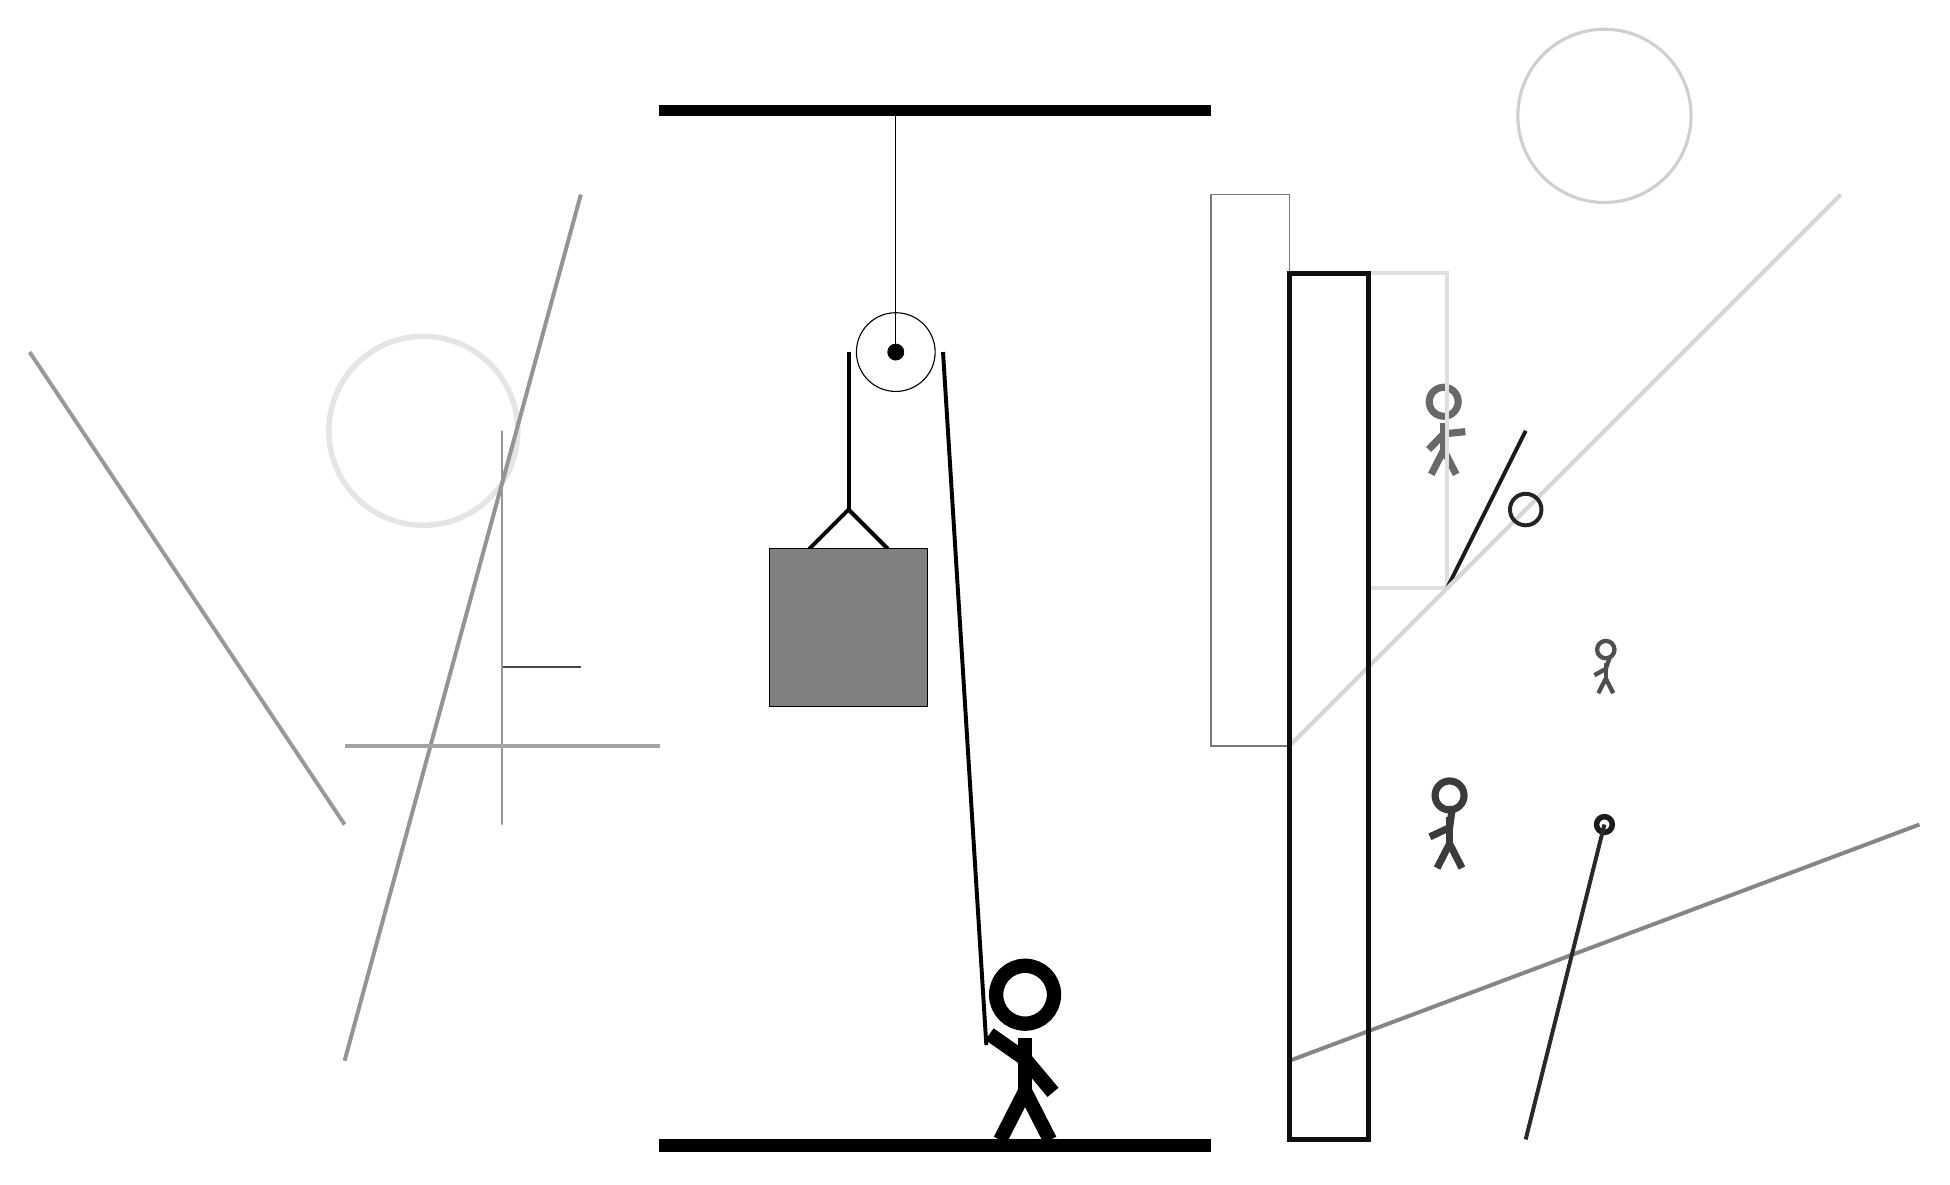
\begin{tikzpicture}
		%%%%% START %%%%%
		
		\draw[fill=black] (-2, 10) rectangle (5, 10.125);
		
		\node[line width=0.2mm, color=black!59] at (8, 6) {\Strichmaxerl[5][46][6]};
		
		\draw [line width=0.2mm, color=black!31](-3, 6) circle (0.0);
		\draw [line width=0.7mm, color=black!89](10, 1) circle (0.1);
		\draw[line width=0.5mm, color=black!12] (7, 8) rectangle (8, 4);
		\node[line width=0.2mm, color=black!69] at (10, 3) {\Strichmaxerl[3][29][71]};
		\draw[line width=0.5mm, color=black!89](8, 4) -- (9, 6);
		\draw [line width=0.7mm, color=black!10](-5, 6) circle (1.2);
		
		\node[line width=0.2mm, color=black!77] at (8, 1) {\Strichmaxerl[5][25][82]};
		\draw[line width=0.5mm, color=black!16](6, 2) -- (13, 9);
		\draw[line width=0.3mm, color=black!72] (-4, 3) rectangle (-3, 3);
		\draw[line width=0.2mm, color=black!53] (5, 9) rectangle (6, 2);
		\draw[line width=0.5mm, color=black!42](-3, 9) -- (-6, -2);
		\draw [line width=0.4mm, color=black!19](10, 10) circle (1.1);
		
		\draw[line width=0.6mm, color=black!79] (6, 6) rectangle (6, 7);
		\draw[line width=0.5mm, color=black!48](6, -2) -- (14, 1);
		\draw[line width=0.5mm, color=black!40](-6, 1) -- (-10, 7);
		
		\draw [line width=0.5mm, color=black!86](9, 5) circle (0.2);
		\draw[line width=0.2mm, color=black!41] (-4, 1) rectangle (-4, 6);
		\draw[line width=0.5mm, color=black!84](10, 1) -- (9, -3);
		\draw[line width=0.5mm, color=black!36](-2, 2) -- (-6, 2);
		\draw[line width=0.6mm, color=black!94] (6, -3) rectangle (7, 8);
		
		
		\draw (1, 7) circle (0.5);
		\draw[fill=black] (1, 7) circle (0.1);
		\draw (1, 10) -- (1, 7);
		
		\draw[line width=0.5mm] (-0.1, 4.5) -- (0.4, 5.0) -- (0.9, 4.5);
		\draw[fill=black!50] (-0.6, 4.5) rectangle (1.4, 2.5);
		
		\draw[line width=0.5mm] (0.4, 7) -- (0.4, 5.0);
		\centerarc[line width=0.5mm](1, 7)(0:180:0.6);
		\draw[line width=0.5mm](1.6, 7) -- (2.15, -1.8);
		
		\node at (2.6, -1.9) {\Strichmaxerl[10][-35][-50]};
		
		\draw[fill=black] (-2, -3) rectangle (5, -3.15);
		
		%%%%% END %%%%%
	\end{tikzpicture}
\end{document}